\documentclass[border=4pt]{standalone}
\usepackage{tikz,amsmath,amssymb}
\usetikzlibrary{arrows.meta,patterns,calc}
% Charte ENSTA
\definecolor{nuit}{HTML}{190F3C}\definecolor{bleu}{HTML}{3746FF}
\definecolor{bleuclair}{HTML}{9BA3FF}\definecolor{corailf}{HTML}{D6455A}
\begin{document}
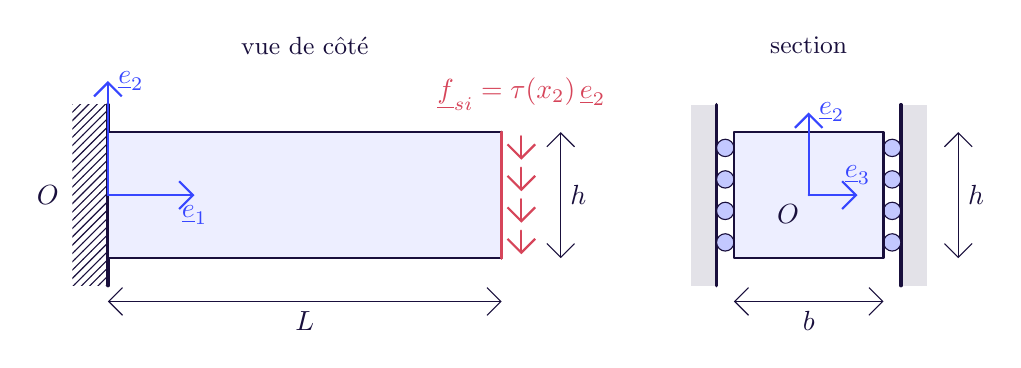
\begin{tikzpicture}[line cap=round,line join=round,>={Straight Barb[length=5pt]},
  cote/.style={<->,nuit,thin}]
  %% ---------- Vue de côté (plan x1, x2) ----------
  \def\L{5}\def\h{1.6}
  % encastrement
  \fill[pattern=north east lines,pattern color=nuit] (-0.45,-1.15) rectangle (0,1.15);
  \draw[very thick,nuit] (0,-1.15) -- (0,1.15);
  % bloc
  \draw[thick,nuit,fill=bleuclair!18] (0,-\h/2) rectangle (\L,\h/2);
  % repère
  \draw[->,thick,bleu] (0,0) -- (1.1,0) node[below] {$\underline{e}_1$};
  \draw[->,thick,bleu] (0,0) -- (0,1.45) node[right] {$\underline{e}_2$};
  \node[nuit,anchor=east] at (-0.5,0) {$O$};
  % chargement f_si = tau(x2) e2 sur x1 = L
  \draw[very thick,corailf] (\L,-\h/2) -- (\L,\h/2);
  \foreach \y in {-0.6,-0.2,0.2,0.6}
    \draw[->,thick,corailf] (\L+0.25,\y+0.15) -- (\L+0.25,\y-0.15);
  \node[corailf,anchor=south] at (\L+0.25,0.95) {$\underline{f}_{si} = \tau(x_2)\,\underline{e}_2$};
  % cotes
  \draw[cote] (0,-1.35) -- (\L,-1.35) node[midway,below] {$L$};
  \draw[cote] (\L+0.75,-\h/2) -- (\L+0.75,\h/2) node[midway,right] {$h$};
  \node[nuit] at (\L/2,1.9) {\small vue de côté};

  %% ---------- Section (plan x3, x2) ----------
  \begin{scope}[xshift=8.9cm]
    \def\b{1.9}
    % parois latérales avec glissement (contact sans frottement)
    \foreach \s in {-1,1} {
      \fill[nuit!12] ({\s*(\b/2+0.22)},-1.15) rectangle ({\s*(\b/2+0.55)},1.15);
      \draw[very thick,nuit] ({\s*(\b/2+0.22)},-1.15) -- ({\s*(\b/2+0.22)},1.15);
      \foreach \y in {-0.6,-0.2,0.2,0.6}
        \draw[nuit,fill=bleuclair!60] ({\s*(\b/2+0.11)},\y) circle (0.11);
    }
    \draw[thick,nuit,fill=bleuclair!18] (-\b/2,-\h/2) rectangle (\b/2,\h/2);
    \draw[->,thick,bleu] (0,0) -- (0.62,0) node[above] {$\underline{e}_3$};
    \draw[->,thick,bleu] (0,0) -- (0,1.05) node[right] {$\underline{e}_2$};
    \node[nuit,anchor=north east] at (0,0) {$O$};
    \draw[cote] (-\b/2,-1.35) -- (\b/2,-1.35) node[midway,below] {$b$};
    \draw[cote] (\b/2+0.95,-\h/2) -- (\b/2+0.95,\h/2) node[midway,right] {$h$};
    \node[nuit] at (0,1.9) {\small section};
  \end{scope}
\end{tikzpicture}
\end{document}
